%  LaTeX support: latex@mdpi.com
%  For support, please attach all files needed for compiling as well as the log file, and specify your operating system, LaTeX version, and LaTeX editor.

%=================================================================
% pandoc conditionals added to preserve backwards compatibility with previous versions of rticles

\documentclass[nutrients,article,submit,moreauthors,pdftex]{Definitions/mdpi}


%% Some pieces required from the pandoc template
\setlist[itemize]{leftmargin=*,labelsep=5.8mm}
\setlist[enumerate]{leftmargin=*,labelsep=4.9mm}


%--------------------
% Class Options:
%--------------------

%---------
% article
%---------
% The default type of manuscript is "article", but can be replaced by:
% abstract, addendum, article, book, bookreview, briefreport, casereport, comment, commentary, communication, conferenceproceedings, correction, conferencereport, entry, expressionofconcern, extendedabstract, datadescriptor, editorial, essay, erratum, hypothesis, interestingimage, obituary, opinion, projectreport, reply, retraction, review, perspective, protocol, shortnote, studyprotocol, systematicreview, supfile, technicalnote, viewpoint, guidelines, registeredreport, tutorial
% supfile = supplementary materials

%----------
% submit
%----------
% The class option "submit" will be changed to "accept" by the Editorial Office when the paper is accepted. This will only make changes to the frontpage (e.g., the logo of the journal will get visible), the headings, and the copyright information. Also, line numbering will be removed. Journal info and pagination for accepted papers will also be assigned by the Editorial Office.

%------------------
% moreauthors
%------------------
% If there is only one author the class option oneauthor should be used. Otherwise use the class option moreauthors.

%---------
% pdftex
%---------
% The option pdftex is for use with pdfLaTeX. Remove "pdftex" for (1) compiling with LaTeX & dvi2pdf (if eps figures are used) or for (2) compiling with XeLaTeX.

%=================================================================
% MDPI internal commands - do not modify
\firstpage{1}
\makeatletter
\setcounter{page}{\@firstpage}
\makeatother
\pubvolume{1}
\issuenum{1}
\articlenumber{0}
\pubyear{2024}
\copyrightyear{2024}
%\externaleditor{Academic Editor: Firstname Lastname}
\datereceived{ }
\daterevised{ } % Comment out if no revised date
\dateaccepted{ }
\datepublished{ }
%\datecorrected{} % For corrected papers: "Corrected: XXX" date in the original paper.
%\dateretracted{} % For corrected papers: "Retracted: XXX" date in the original paper.
\hreflink{https://doi.org/} % If needed use \linebreak
%\doinum{}
%\pdfoutput=1 % Uncommented for upload to arXiv.org
%\CorrStatement{yes}  % For updates


%=================================================================
% Add packages and commands here. The following packages are loaded in our class file: fontenc, inputenc, calc, indentfirst, fancyhdr, graphicx, epstopdf, lastpage, ifthen, float, amsmath, amssymb, lineno, setspace, enumitem, mathpazo, booktabs, titlesec, etoolbox, tabto, xcolor, colortbl, soul, multirow, microtype, tikz, totcount, changepage, attrib, upgreek, array, tabularx, pbox, ragged2e, tocloft, marginnote, marginfix, enotez, amsthm, natbib, hyperref, cleveref, scrextend, url, geometry, newfloat, caption, draftwatermark, seqsplit
% cleveref: load \crefname definitions after \begin{document}

%=================================================================
% Please use the following mathematics environments: Theorem, Lemma, Corollary, Proposition, Characterization, Property, Problem, Example, ExamplesandDefinitions, Hypothesis, Remark, Definition, Notation, Assumption
%% For proofs, please use the proof environment (the amsthm package is loaded by the MDPI class).

%=================================================================
% Full title of the paper (Capitalized)
\Title{Association between substitution of red meat with legumes and risk of primary liver cancer in UK Biobank participants: A prospective cohort study}

% MDPI internal command: Title for citation in the left column
\TitleCitation{Association between substitution of red meat with legumes and risk of primary liver cancer in UK Biobank participants: A prospective cohort study}

% Author Orchid ID: enter ID or remove command
%\newcommand{\orcidauthorA}{0000-0000-0000-000X} % Add \orcidA{} behind the author's name
%\newcommand{\orcidauthorB}{0000-0000-0000-000X} % Add \orcidB{} behind the author's name


% Authors, for the paper (add full first names)
\Author{Niels Bock$^{1}$\href{https://orcid.org/0009-0005-7373-1589}
{\orcidicon}, Fie Langmann$^{1}$\href{https://orcid.org/0000-0003-3474-9346}
{\orcidicon}, Luke W. Johnston$^{1, 2}$\href{https://orcid.org/0000-0003-4169-2616}
{\orcidicon}, Daniel B. Ibsen$^{1, 2}$\href{https://orcid.org/0000-0002-7038-4770}
{\orcidicon}, Christina C. Dahm$^{1, *}$\href{https://orcid.org/0000-0003-0481-2893}
{\orcidicon}}


%\longauthorlist{yes}


% MDPI internal command: Authors, for metadata in PDF
\AuthorNames{Niels Bock, Fie Langmann, Luke W. Johnston, Daniel B. Ibsen, Christina C. Dahm}

% MDPI internal command: Authors, for citation in the left column
%\AuthorCitation{Lastname, F.; Lastname, F.; Lastname, F.}
% If this is a Chicago style journal: Lastname, Firstname, Firstname Lastname, and Firstname Lastname.
\AuthorCitation{Bock, N; Langmann, F; Johnston, LW; Ibsen, DB; Dahm, CC}

% Affiliations / Addresses (Add [1] after \address if there is only one affiliation.)
\address{%
$^{1}$ \quad Department of Public Health,
Aarhus University,
Aarhus, Denmark; \\
$^{2}$ \quad Steno Diabetes Center Aarhus,
Aarhus University Hospital,
Aarhus N, Denmark; \\
}

% Contact information of the corresponding author
\corres{Correspondence: \href{mailto:CCD@ph.au.dk}{\nolinkurl{CCD@ph.au.dk}}.}

% Current address and/or shared authorship








% The commands \thirdnote{} till \eighthnote{} are available for further notes

% Simple summary

%\conference{} % An extended version of a conference paper

% Abstract (Do not insert blank lines, i.e. \\)
\abstract{Primary liver cancer is globally on the rise, partially due to poor diets and
sedentary lifestyles. Shifting to more plant-based diets may lower the risk.
We aimed to estimate the effect of replacing total red meat, unprocessed red
meat and processed red meat with legumes on primary liver cancer in a
free-living population. We analyzed data from 126,744 UK Biobank participants
who completed \(\geq\) two 24-hour diet recalls. Baseline characteristics were
collected from the initial assessment visit. Information on liver cancer
diagnoses was collected via external linkage to inpatient hospital episodes or
central cancer registries. Cox proportional hazards regression models were
used to estimate substitution of 15 g/day of legumes with 15 g/day of total
red meat, unprocessed red meat or processed red meat on liver cancer risk,
using the leave-one-out food substitution model. During a median follow-up
time of 11.1 years, 173 participants developed liver cancer. In the fully
adjusted models, no association was observed when substituting 15 g/day of
legumes with total red meat (HR: 1.02 (95\% CI 0.96-1.08)), unprocessed red
meat (HR: 1.00 (95\% CI 0.94-1.06)) or processed red meat (HR: 1.09 (95\% CI
0.99-1.21)). Overall, little evidence of an association between replacing red
meat with legumes and liver cancer was observed. Further research in other
study populations with longer follow-up time is warranted.}


% Keywords
\keyword{food substitutions; liver cancer; red meat; legumes.}

% The fields PACS, MSC, and JEL may be left empty or commented out if not applicable
%\PACS{J0101}
%\MSC{}
%\JEL{}

%%%%%%%%%%%%%%%%%%%%%%%%%%%%%%%%%%%%%%%%%%
% Only for the journal Diversity
%\LSID{\url{http://}}

%%%%%%%%%%%%%%%%%%%%%%%%%%%%%%%%%%%%%%%%%%
% Only for the journal Applied Sciences

%%%%%%%%%%%%%%%%%%%%%%%%%%%%%%%%%%%%%%%%%%

%%%%%%%%%%%%%%%%%%%%%%%%%%%%%%%%%%%%%%%%%%
% Only for the journal Data



%%%%%%%%%%%%%%%%%%%%%%%%%%%%%%%%%%%%%%%%%%
% Only for the journal Toxins


%%%%%%%%%%%%%%%%%%%%%%%%%%%%%%%%%%%%%%%%%%
% Only for the journal Encyclopedia


%%%%%%%%%%%%%%%%%%%%%%%%%%%%%%%%%%%%%%%%%%
% Only for the journal Advances in Respiratory Medicine
%\addhighlights{yes}
%\renewcommand{\addhighlights}{%

%\noindent This is an obligatory section in “Advances in Respiratory Medicine”, whose goal is to increase the discoverability and readability of the article via search engines and other scholars. Highlights should not be a copy of the abstract, but a simple text allowing the reader to quickly and simplified find out what the article is about and what can be cited from it. Each of these parts should be devoted up to 2~bullet points.\vspace{3pt}\\
%\textbf{What are the main findings?}
% \begin{itemize}[labelsep=2.5mm,topsep=-3pt]
% \item First bullet.
% \item Second bullet.
% \end{itemize}\vspace{3pt}
%\textbf{What is the implication of the main finding?}
% \begin{itemize}[labelsep=2.5mm,topsep=-3pt]
% \item First bullet.
% \item Second bullet.
% \end{itemize}
%}


%%%%%%%%%%%%%%%%%%%%%%%%%%%%%%%%%%%%%%%%%%


% tightlist command for lists without linebreak
\providecommand{\tightlist}{%
  \setlength{\itemsep}{0pt}\setlength{\parskip}{0pt}}

% From pandoc table feature
\usepackage{longtable,booktabs,array}
\usepackage{calc} % for calculating minipage widths
% Correct order of tables after \paragraph or \subparagraph
\usepackage{etoolbox}
\makeatletter
\patchcmd\longtable{\par}{\if@noskipsec\mbox{}\fi\par}{}{}
\makeatother
% Allow footnotes in longtable head/foot
\IfFileExists{footnotehyper.sty}{\usepackage{footnotehyper}}{\usepackage{footnote}}
\makesavenoteenv{longtable}


\usepackage{caption}
\captionsetup{font=small,justification=raggedright,singlelinecheck=false}
\usepackage{longtable, fancyhdr}
\usepackage{booktabs}
\usepackage{caption}
\usepackage{longtable}
\usepackage{rotating}
\usepackage{colortbl}
\usepackage{array}
\usepackage{anyfontsize}
\usepackage{multirow}

\begin{document}



%%%%%%%%%%%%%%%%%%%%%%%%%%%%%%%%%%%%%%%%%%

\hypertarget{sec1}{%
\section{Introduction}\label{sec1}}

Hepatocellular carcinoma (HCC) is the sixth most common cancer in the
world and the third leading cause of cancer-related death with viral
hepatitis being the leading risk factor \citep{Massarweh2017}. In
low-infection populations, modifiable risk factors, such as dietary
habits, may play an increasing role in HCC pathogenesis as non-alcoholic
fatty liver disease (NAFLD) has become the leading cause of liver
cirrhosis \citep{Younossi2016, Younossi2020} that may in turn progress to
HCC. A western dietary pattern high in fats and red meats and
concurrently low in fruits, vegetables, and whole grains has been
associated with NAFLD progression \citep{Guo2022}. The prevalence of
NAFLD-related HCC cases is an increasing global problem \citep{Younossi2016}.
It is estimated that the prevalence of NAFLD-related HCC in the US will
increase by 146\%, while incident NAFLD-related HCC cases will increase
by 137\% in 2030 \citep{Estes2018}.

The second most common primary liver cancer is the intrahepatic
cholangiocarcinoma (ICC) \citep{Khan2019}. While HCC emerges from the liver
parenchyma, ICC emerges from the bile duct. Despite being a relatively
rare cancer, ICC is characterized by its aggressiveness, late diagnosis
and poor survival \citep{kirstein2016}. It is estimated that the incidence of
ICC is increasing in populations that are not burdened by known
infectious and environmental risk factors \citep{Bergquist2015}. Recent
meta-analyses of observational studies and clinical trials have shown a
significant adverse association between NAFLD and ICC
\citep{Wongjarupong2017, corrao2020}.

The impact of specific food groups on liver cancer risk is not well
known. Observational studies suggest that intake of coffee, vegetables
and whole grains may lower HCC risk \citep{zhang2013, yang2014, Liu2021, Bhurwal2020}. The protective properties of these foods are proposed to
be their content of dietary fibers and polyphenols, which are also
defining components of legumes \citep{rebello2014}. Polyphenols such as
phenolic acid and flavonoids inhibit free radical and may thus protect
human tissues against oxidative stress \citep{scalbert2002, bouchenak2013}.
Phytic acid and saponins may have anti-carcinogenic properties via
regulation of the cell cycle and enzymes involved in the apotosis
pathway, and inhibition of the metastatic potential of tumors
\citep{Vucenik2006, campos-vega2010, rebello2014}.The health benefits of
legumes extend to improved glycemic control and hypotensive and
anticarcinogenic properties with observed inverse associations with
cardiovascular disease and colorectal cancer \citep{viguiliouk2019, jin2022}. Two large prospective cohort studies (N = 130,000-500,000, n
event = 298-940) found evidence of inverse associations between legume
consumption and risk of HCC \citep{zhang2013, Liu2021}. However, replacement
foods were not specified in these studies, which fails to reflect that a
higher intake of one food is at the expense of a concomitantly lower
intake of another food. On the contrary, processed red meat intake, but
not unprocessed red meat intake, was associated with an increased risk
of HCC in two large cohorts (N = 50,000-120,000, n events = 163),
suggesting that the processing of red meat may augment the carcinogenic
effects on the liver tissues \citep{Ma2019}. Processed red meat is classified
as ``carcinogenic to humans'' and unprocessed red meat as a possible
carcinogen by the International Agency for Research on Cancer
\citep{Bouvard2015}. Studies on substituting animal-based proteins with
plant-based proteins are important if we are to lower the climate
impacts of our diets \citep{RN71}. While previous research has investigated
and found protective effects when substituting animal-based proteins
with plant-based proteins in relations to NAFLD \citep{Zhang2023}, research
on substituting meats with legumes in relation to risk of HCC and ICC is
sparse. This leaves a substantial gap in the current knowledge on the
beneficial effects on primary liver cancer from substituting red meat
with legumes.

The low incidence of liver cancer in populations not burdened by viral
hepatitis complicates observational prospective research designs;
nonetheless, the prospects of the burden of liver cancer on public
health warrant investigation of preventative measures. Thus, the main
aim of this study was to estimate the association between replacing
unprocessed red meat, processed red meat and total red meat with legumes
on primary liver cancer in a large free-living population.

\hypertarget{sec2}{%
\section{Materials and Methods}\label{sec2}}

\noindent The protocol for this study was written prior to conducting
the analysis. It is available on the archive Zenodo \citep{protocol}. Some
changes were made to the final analysis plan due to lack of power to
conduct subgroup and mediation analyses.

\hypertarget{subsec1}{%
\subsection{Study population}\label{subsec1}}

The UK Biobank is a population-based prospective cohort initiated in
2006 \citep{sudlow2015}. During 2006-2010, more than 500,000 participants,
aged 40-69, were recruited and visited designated assessment centres
across the UK. Participants provided information about age, sex,
sociodemographic factors and lifestyle factors via touch screen
questionnaires, and computer-assisted interviews. Anthropometric data
were collected via physical measurements \citep{RN113}.

\hypertarget{subsec2}{%
\subsection{Dietary assessment}\label{subsec2}}

A web-based 24-hour dietary recall was administered at the end of the
initial assessment visit for the last 70,000 recruited participants
\citep{RN115}. From February 2011 to April 2012, 320,000 participants who had
provided an e-mail address were invited on four separate occasions to
complete the 24-hour dietary recall, the Oxford WebQ, of which 210,947
participants completed at least one. The Oxford WebQ covered 206 food
items and 32 beverage items commonly consumed in the UK. Intakes were
reported in standard units of measurements, e.g., servings, cups,
slices, etc. with intake categories ranging from 0 to 3+ units
\citep{piernas2021}. The Oxford WebQ has been validated against
interviewer-based 24-hour dietary recalls showing acceptable
correlations for total energy intake and most nutrients, and biomarkers
showing acceptable correlations between the average values of two or
more Oxford WebQs and estimated true intakes of total energy, total
sugar, potassium and protein \citep{Liu2011, Greenwood2019}.

A total of 79 food categories and 14 beverage categories from the Oxford
WebQ has previously been defined using the UK National Diet and
Nutrition Survey categories \citep{piernas2021}. We used these food and
beverage groups when defining the food groups used in the substitution
analyses (Table S1). Legumes were defined as legumes and dietary pulses,
baked beans, tofu-based products, peas, hummus, soy drinks, and
soy-based desserts and yogurt. Unprocessed red meat intake was defined
as intake of beef, pork, lamb, or other meat, including offal. Processed
red meat intake was defined as sausages, bacon (with and without fat),
ham, or liver paté. Total red meat was the combination of unprocessed
and processed red meat. Other food groups included were animal-based
foods, unhealthy plant-based foods, healthy plant-based foods, and
alcoholic beverages (Table S1). Animal-based and healthy and unhealthy
plant-based food foods were grouped based on plant-based diet indices
from previous studies \citep{Thompson2023, Heianza2021, Satija2017, Satija2016}.

As a single 24-hour dietary recall does not assess habitual dietary
intake and variation in diet over time at an individual level
\citep{thompson2013, gurinovic2017}, only participants who completed two or
more Oxford WebQs were eligible for inclusion in this study. Baseline
food intakes were defined as average intakes from the reported 24-hour
diet recalls.

\hypertarget{subsec3}{%
\subsection{Liver cancer assessment}\label{subsec3}}

Liver cancer was defined according to ICD-10 diagnosis codes C22.0 for
Hepatocellular carcinoma (HCC) or C22.1 for Intrahepatic
cholangiocarcinoma (ICC) and ICD-9 diagnosis codes 1550 Malignant
neoplasm of liver, primary or 1551 Malignant neoplasm of intrahepatic
bile ducts. Incident and prevalent cases of liver cancer and
corresponding diagnosis dates were obtained via external linkage to
central cancer registries or hospital inpatient episodes \citep{RN112, RN114}.

\hypertarget{subsec4}{%
\subsection{Assessment of confounders}\label{subsec4}}

Confounders were defined \emph{a priori} from a review of the literature and
illustrated using directed acyclic graphs (Figure S1). The following
confounding variables were selected: age, sex, educational level,
Townsend deprivation index (TDI), living alone, physical activity,
smoking, alcohol intake, and waist circumference. Information on all
confounders except age was collected at the initial assessment visit
before the start of follow-up.

\hypertarget{subsec6}{%
\subsection{Statistical analysis}\label{subsec6}}

Baseline characteristics and intake of food groups of all included
participants and participants who developed liver cancer were described
using standard summary statistics. Continuous variables were described
with medians and interquartile range (IQR, 25th-75th percentiles) and
categorical variables in total numbers (n) and percentage (\%). Intake of
food groups were described as g/day.

Multivariable-adjusted Cox proportional hazards regression models were
used to estimate hazard ratios (HR) with corresponding 95\% confidence
intervals (CI) with age as the underlying timescale. Participants were
followed from the date of their last completed Oxford WebQ until the
occurrence of the event of interest or due to right censoring, whichever
came first. Participants were right censored in the event of death, loss
to follow-up, or administrative end of follow-up (October 31, 2022).

The substitution analyses were conducted by modeling replacement of an
equal mass of meat with legumes. The portion size of the substitution
was set to 15 g/day of legumes for 15 g/day of red meat to ensure that
substitutions were below the mean intake of any of the substituted food
groups in the cohort. The substitutions were modeled using the
leave-one-out-approach in which variables for every food group intake
along with a variable for total food intake were included, except the
food group that were to be substituted \citep{Ibsen2021}. To estimate
replacing of 15 g/day of all red meats (unprocessed and processed) with
15 g/day of legumes, the following model was defined:

{\small
\begin{align}
\log(h(t;x)) &= \log(h_0(t)) + \beta_1 \text{Legumes (15 g/day)} \hspace{0.5em} + \nonumber \\
&\quad \hspace{0.5em} \beta_2 \text{Total food intake (g/day)} + \beta_3 \text{´Other food groups (g/day)} + \beta_4 \text{´Covariates}
\end{align}
}

\noindent When substituting only unprocessed red meat with legumes,
processed red meat was added to the model:

{\small
\begin{align}
\log(h(t;x)) &= \log(h_0(t)) + \beta_1 \text{Legumes (15 g/day)} + \beta_2 \text{Processed red meat (15 g/day)} \hspace{0.5em} + \nonumber \\
&\quad \hspace{0.5em} \beta_3 \text{Total food intake (g/day)} + \beta_4 \text{´Other food groups (g/day)} + \beta_5 \text{´Covariates}
\end{align}
}

\noindent When substituting only processed red meat with legumes,
unprocessed red meat was added to the model:

{\small
\begin{align}
\log(h(t;x)) &= \log(h_0(t)) + \beta_1 \text{Legumes (15 g/day)} + \beta_2 \text{Unprocessed red meat (15 g/day)} \hspace{0.5em} + \nonumber \\
&\quad \hspace{0.5em} \beta_3 \text{Total food intake (g/day)}  + \beta_4 \text{´Other food groups (g/day)} + \beta_5 \text{´Covariates}
\end{align}
}

\noindent The performance of the leave-one-out model when modeling equal
mass substitutions has been validated against simulated data
\citep{Tomova2022}.

Two levels of adjustments were added to the substitution model. Model 1
was minimally adjusted for age (as the underlying timescale) total
weight of food and beverage intake (g/day), and all other food groups
(g/day) to fit the substitution model. To account for differences in
baseline risks, model 1 was additionally stratified on age at
recruitment (\textless45, 45-49, 50-54, 55-59, 60-64 and \(\geq\) 65), attended
assessment centre, and sex (male, female). Model 2 was further adjusted
for educational level (high: College or University degree, intermediate:
A levels/AS levels, O levels/GCSEs, or equivalent, low: none of the
previous mentioned), Townsend deprivation index (continuous), living
alone (yes, no), physical activity (above/below the 2017 UK Physical
activity guidelines of 150 minutes of moderate activity per week or 75
minutes of vigorous activity, or unknown), smoking (pack years as a
proportion of lifespan exposed to smoking, continuous), alcohol intake
(g/day, continuous), and waist circumference (cm, continuous). The
included covariates, including food groups, were grouped to ensure
adequate power in the analyses to discover any associations between the
exposure and outcome of interest and were guided by our \emph{a priori}
assumptions \citep{protocol}. Assumptions of proportional hazards were
checked using Schoenfeld residuals and showed no violations.

In secondary analyses, each cancer type was analysed separately to
evaluate if the pooling of HCC and ICC as one outcome in the main
analysis was justified. Furthermore, to estimate the association of
legume intake with liver cancer, not specifying the substitution, legume
consumers (divided into quartiles) were compared to non-consumers.

To evaluate the robustness of the main analyses, sensitivity analyses
were performed on subsamples of participants by excluding those with
high alcohol intake (exclusion of the upper decile of alcohol intake
(g/day) by sex), implausible energy intake (exclusion of participants
below the 2.5th percentile and above the 97.5th percentile of energy
intake (kJ/day) by sex), any liver disease before baseline, any type of
cancer before baseline, and fewer than three completed Oxford WebQs. As
neither the central cancer registries nor the hospital inpatient
registries were complete, liver cancer diagnoses retrieved from death
registries, which were updated more recently, were included in a
sensitivity analysis to test for outcome misclassification. Further, one
of the causal assumptions was that anthropometry confounded the causal
relationship between replacing red meat with legumes and liver cancer;
however, arguments exist giving support to anthropometry being a
mediator between diet and health outcomes. Thus, to test for erroneously
conditioning on a potential mediator, a sensitivity analysis was
adjusted following model 2 but without waist circumference. Lastly,
sensitivity analyses omitting soy milk from the estimated daily legume
intake were conducted, as soy milk is unlikely to culinarily replace red
meat. All sensitivity analyses were modeled as the fully adjusted models
in the main analyses.

All analyses were conducted in R version 4.4.0 (2024-04-24) with a
significance level of 5\%. The code is structured in a reproducible
manner using the targets R package \citep{landau2021} and is available at
\url{https://github.com/steno-aarhus/legliv}.

\hypertarget{sec3}{%
\section{Results}\label{sec3}}

After excluding participants with liver cancer before baseline,
participants lost to follow-up before baseline, and participants with
errors in dietary data, 126,744 participants who had completed two or
more Oxford WebQs remained (Figure \ref{fig:fig1}).

\begin{figure*}

{\centering 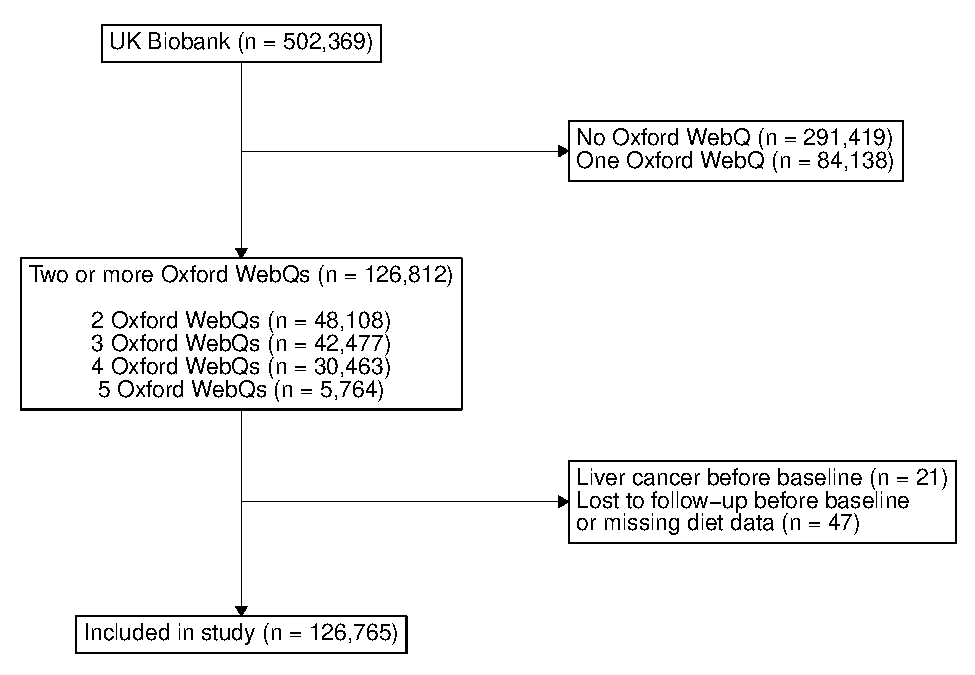
\includegraphics[width=1\linewidth,]{legliv-nutrients_files/figure-latex/fig1-1} 

}

\caption{Flowchart of included participants. Not all UK Biobank participants were invited to complete an Oxfords WebQ. Only the last 70,000 participants to visit an assessment center were asked to complete an Oxford WebQ at the end of their visit. Further Oxford WebQs were sent to ~320,000 participants who provided an e-mail address.}\label{fig:fig1}
\end{figure*}

During a median follow-up time of 11.1 years, 173 participants developed
liver cancer of which 73 were HCC and 100 were ICC. Those who developed
liver cancer were older at baseline, were more likely to be male, have a
higher waist circumference, be less physically active, and fewer had
never smoked, compared to all included participants (Table
\ref{tab:baseline}).

\begin{table}[t]
\caption{\label{tab:baseline}\textbf{Baseline characteristics of UK Biobank participants who completed \(\geq\) 2 Oxford WebQ dietary recalls.}} 
\fontsize{9.0pt}{10.8pt}\selectfont
\begin{tabular*}{1\linewidth}{@{\extracolsep{\fill}}lcc}
\toprule
 & \textbf{Cohort} & \textbf{Liver cancer} \\ 
\cmidrule(lr){2-2} \cmidrule(lr){3-3}
\textbf{Variable} & \textbf{N = 126,744}\textsuperscript{\textit{1}} & \textbf{N = 173}\textsuperscript{\textit{1}} \\ 
\midrule\addlinespace[2.5pt]
{\bfseries Age, years} & 60 (53, 65) & 64.0 (60.0, 68.0) \\ 
{\bfseries Sex} &  &  \\ 
    Female & 70,659 (56\%) & 65 (38\%) \\ 
    Male & 56,085 (44\%) & 108 (62\%) \\ 
{\bfseries Educational level}\textsuperscript{\textit{2}} &  &  \\ 
    High & 59,416 (47\%) & 76 (44\%) \\ 
    Intermediate & 41,817 (33\%) & 52 (30\%) \\ 
    Low & 25,472 (20\%) & 45 (26\%) \\ 
    Missing & 39 &  \\ 
{\bfseries Townsend Deprivation Index} & -2.4 (-3.8, 0.0) & -2.6 (-3.7, -0.7) \\ 
    Missing & 149 &  \\ 
{\bfseries Living alone} & 22,658 (18\%) & 34 (20\%) \\ 
    Missing & 171 &  \\ 
{\bfseries Physical activity}\textsuperscript{\textit{3}} &  &  \\ 
    Above & 58,111 (46\%) & 61 (35\%) \\ 
    Below & 50,712 (40\%) & 79 (46\%) \\ 
    Unknown & 17,921 (14\%) & 33 (19\%) \\ 
{\bfseries Smoking} &  &  \\ 
    Never & 72,583 (57\%) & 75 (43\%) \\ 
    Ever & 54,122 (43\%) & 98 (57\%) \\ 
    Missing & 39 &  \\ 
{\bfseries Alcohol intake, g/day} & 11 (0, 26) & 11 (0, 29) \\ 
{\bfseries Waist circumference, cm} & 88 (79, 97) & 98 (89, 107) \\ 
    Missing & 168 &  \\ 
\bottomrule
\end{tabular*}
\begin{minipage}{\linewidth}
\textsuperscript{\textit{1}}Median (IQR) for continuous variables; n (\%) for categorical variables\\
\textsuperscript{\textit{2}}High: College or University degree;
Intermediate: A levels/AS levels, O levels/GCSEs, or equivalent;
Low: none of the previously mentioned.\\
\textsuperscript{\textit{3}}Above or below the 2017 UK Physical activity guidelines of 150 minutes of moderate activity per week or 75 minutes of vigorous activity.\\
\end{minipage}
\end{table}

\noindent Mean daily energy and total food intakes as well as daily
intake of all specified food groups in grams are presented in Table
\ref{tab:diet}.

\begin{table}[t]
\caption{\label{tab:diet}\textbf{Daily dietary intake of food groups, total food, and total energy intake in UK Biobank participants who completed \(\geq\) 2 Oxford WebQ dietary recalls.}} 
\fontsize{9.0pt}{10.8pt}\selectfont
\begin{tabular*}{1\linewidth}{@{\extracolsep{\fill}}lcc}
\toprule
 & \textbf{Cohort} & \textbf{Liver cancer} \\ 
\cmidrule(lr){2-2} \cmidrule(lr){3-3}
\textbf{Daily food intake} & \textbf{N = 126,744}\textsuperscript{\textit{1}} & \textbf{N = 173}\textsuperscript{\textit{1}} \\ 
\midrule\addlinespace[2.5pt]
\multicolumn{3}{l}{{\bfseries Total food intake}} \\ 
\midrule\addlinespace[2.5pt]
Energy, kJ & 8,430 (7,179, 9,856) & 8,579 (7,413, 10,048) \\ 
Weight, g & 3,144 (2,720, 3,621) & 3,162 (2,737, 3,659) \\ 
\midrule\addlinespace[2.5pt]
\multicolumn{3}{l}{{\bfseries Food groups, g/day}} \\ 
\midrule\addlinespace[2.5pt]
Legumes & 11 (0, 34) & 8 (0, 35) \\ 
Red and processed meat & 53 (15, 86) & 60 (30, 95) \\ 
Red meat & 30 (0, 60) & 45 (0, 73) \\ 
Processed meat & 9 (0, 30) & 8 (0, 31) \\ 
Other animal-based foods\textsuperscript{\textit{2}} & 475 (361, 603) & 448 (322, 604) \\ 
Healthy plant-based foods\textsuperscript{\textit{3}} & 1,806 (1,454, 2,198) & 1,791 (1,365, 2,158) \\ 
Unhealthy plant-based foods\textsuperscript{\textit{4}} & 472 (324, 662) & 491 (365, 698) \\ 
Alcoholic beverages & 132 (0, 342) & 144 (0, 375) \\ 
\bottomrule
\end{tabular*}
\begin{minipage}{\linewidth}
\textsuperscript{\textit{1}}Median (Q1, Q3)\\
\textsuperscript{\textit{2}}Other animal-based foods include poultry, fish, dairy, eggs, and mixed dishes with animal products.\\
\textsuperscript{\textit{3}}Healthy plant-based foods include whole grains, vegetables, fruits, nuts, plant oils, and beverages (coffee, tea, water).\\
\textsuperscript{\textit{4}}Unhealthy plant-based foods include refined grains, potatoes, mixed vegetarian dishes, sweets and snacks, fruit juice, and sugar sweetened beverages.\\
\end{minipage}
\end{table}

No evidence of associations was found for substituting 15 g/day of
legumes with 15 g/day of total red meat, unprocessed red meat, or
processed red meat and risk of primary liver cancer in Model 1 (Table
\ref{tab:main}: total red meat:
HR: 0.99, 95\% CI: 0.93-1.05;
unprocessed red meat:
HR: 0.97, 95\% CI: 0.91-1.03;
processed red meat:
HR: 1.04, 95\% CI: 0.94-1.15).
The estimated associations changed minimally with further adjustments.
There was weak evidence of an association between replacement of
processed red meat with legumes
(HR: 1.09, 95\% CI: 0.99-1.21;
Table \ref{tab:main}).

\begin{table}[b]
\caption{\label{tab:main}\textbf{Replacing 15 g/day of total red meat, unprocessed red meat, and processed meat with legumes and hazard ratios and 95\% confidence intervals for primary liver cancer.}} 
\fontsize{9.0pt}{10.8pt}\selectfont
\begin{tabular*}{1\linewidth}{@{\extracolsep{\fill}}lcc}
\toprule
 & {\bfseries \textbf{Model 1}}\textsuperscript{\textit{1}} & {\bfseries \textbf{Model 2}}\textsuperscript{\textit{2}} \\ 
\cmidrule(lr){2-2} \cmidrule(lr){3-3}
\textbf{15 g/day of legumes replacing:} & \textbf{HR} \textbf{(95\% CI)} & \textbf{HR} \textbf{(95\% CI)} \\ 
\midrule\addlinespace[2.5pt]
Total red meat & 0.99 (0.93-1.05) & 1.02 (0.96-1.08) \\ 
Unprocessed red meat & 0.97 (0.91-1.03) & 1.00 (0.94-1.06) \\ 
Processed red meat & 1.04 (0.94-1.15) & 1.09 (0.99-1.21) \\ 
\bottomrule
\end{tabular*}
\begin{minipage}{\linewidth}
\textsuperscript{\textit{1}}Multivariate Cox proportional hazards regression model adjusted for age (as underlying timescale), other food groups, and total food intake, and additionally stratified on sex, age, and attended assessment centre.\\
\textsuperscript{\textit{2}}Further adjusted for educational level, Townsend deprivation index, living alone, physical activity, smoking, alcohol intake, and waist circumference.\\
\end{minipage}
\end{table}

In secondary analyses, when analyzing the associations between
replacement of red meat with legumes and HCC or ICC separately, weak
evidence of a higher risk of HCC was observed (Table S2, total red meat:
HR: 1.06, 95\% CI: 0.97-1.16;
unprocessed red meat:
HR: 1.04, 95\% CI: 0.95-1.15;
processed red meat:
HR: 1.10, 95\% CI: 0.96-1.27).
This association was opposite and inverse for replacement of total red
meat and unprocessed red meat and ICC (total red meat:
HR: 0.97, 95\% CI: 0.89-1.05;
unprocessed red meat:
HR: 0.94, 95\% CI: 0.87-1.02)
but not for processed red meat
(HR: 1.07, 95\% CI: 0.93- 1.23,
Table S2). The magnitude or direction of associations were not
significantly different across strata of liver cancer types.

In the adjusted non-substitution analysis, only the first quartile of
legume intake (mean intake 6.3 grams/day) was associated with a lower
risk of liver cancer, compared to no intake
(HR: 0.60, 95\% CI: 0.36-0.99);
no associations were observed for quartiles 2, 3 or 4 compared to no
intake (Table S3).

In sensitivity analyses, excluding participants based on high alcohol
intake, implausible energy intake, any liver disease or cancer before
baseline, or fewer than 3 completed Oxford WebQs did not alter the
estimates appreciably. Similar results were also found when including
death registries as a source of liver cancer cases and when excluding
waist circumference from the fully adjusted analysis and soy milk from
the food substitutions (Table S4).

\hypertarget{sec4}{%
\section{Discussion}\label{sec4}}

Contrary to our hypothesis, this study showed little evidence of an
association between replacing 15 g/day of unprocessed or processed red
meat with legumes on risk of primary liver cancer. The estimates were
robust to sensitivity analyses. When investigating liver cancer types
separately, replacing total red meat and unprocessed red meat with
legumes showed some weak evidence of an inverse association with ICC but
with wide confidence intervals. The results for legume intake without
specified substitutions did not show a clear pattern of associations.

The prospective longitudinal design of this study established
temporality between the diet exposure and liver cancer outcome, and the
large sample size enabled analyses of a rare cancer. Further, our
specified substitution analyses have some strengths in contrast to
traditional methods in nutritional epidemiology through examining the
association of consuming a food or nutrient while holding all other
foods constant. The substitution is easily interpretable and reflects
the implications that a higher intake of a food is at the expense of a
lower intake of another food. A limitation of this research design was
that the low intake of the substituted foods in this population
restricted the size of the substitution, which may in turn have
restricted findings of clinical relevance.

Information on dietary intake was collected using self-reported 24-hour
diet recalls, which may have introduced measurement error partly due to
the limited ability of 24-hour recalls to estimate habitual dietary
intake. The lack of subsequently administered Oxford WebQs made it
impossible to adjust for dietary changes during the study time. However,
estimates were robust to exclusion of participants with fewer than three
completed Oxford WebQs, indicating that increasing number of dietary
measurements to account for some of the natural fluctuations in dietary
intake over time made little difference to our results. A validation
study of the Oxford WebQ found person-specific biases for correlation
with true intakes for some nutrients, particularly for participants with
a higher BMI \citep{Greenwood2019}. Adjustment for BMI was not included in
this current study. However, adjusting for waist circumference did not
change the estimates appreciably, indicating that such errors do not
explain our results. Finally, by specifying that the dietary exposure
was collected on at least two occasions, the study population suffered
considerable attrition. This is unlikely to be completely at random, and
most likely resulted in a study population with greater focus on their
dietary habits compared to the general population. For example, the mean
intake of processed meat was low in our study population. If a diet
consisting of higher intakes of healthier plant-based foods is
associated with lower liver cancer incidence, our study population may
be at lower risk overall, thus reducing the power of our study to detect
an association.

Registries used to determine a diagnosis of liver cancer were incomplete
or not up-to-date at the time of analysis \citep{RN112}. Data from external
providers, such as the NHS England, NHS Central Register or National
Records of Scotland, were estimated to be mostly complete by the UK
Biobank at various dates, ranging from 31 December 2016 for cancer data
from Wales to 31 October 2022 for hospital inpatient data from England
\citep{RN114}. This could introduce misclassification of the outcome, as
individuals with liver cancer may not be identified as cases. However,
the estimates were robust in a sensitivity analysis that included death
registries as an additional source of liver cancer diagnoses to
accommodate missing outcome events. Incorrectly classifying non-cases as
cases would lead to attenuation of our results, but this is unlikely due
to register linkage. Though health registries may have been only
partially up to date, using registries almost eliminates selection bias
due to loss to follow-up.

The relatively low number of events limited the possibility to adjust
for confounding factors. Excessive adjustment parameters per event can
compromise the validity of the multivariable Cox regression model,
potentially causing biased estimates. To ensure statistical validity, at
least 10 events per variable were aimed for in the main analysis by
limiting the number of adjustment levels, using fewer and broader food
groups, and fewer levels for categorical covariates. This approach was
guided by our \emph{a priori} causal assumptions. Although this method helped
maintain statistical validity, it may have increased residual
confounding by diluting the importance of specific food groups.
Additionally, risk factors that could not be adjust for, such as
aflatoxin B1, a known liver carcinogen, may have contributed to
additional residual confounding.

Contrary to our hypothesis, replacing processed red meat with legumes
was associated with a non-significant increase in risk of primary liver
cancer, with a greater effect size compared to unprocessed red meat.
This pattern persisted across all sensitivity analyses. However, the
estimates for processed red meat were labeled with less confidence,
partly due to the low median intake. The findings of this current study
align with other research in the UK Biobank, where unprocessed red meat
intake was associated with a non-significant increase in liver cancer
risk, with a greater effect size than processed meat (both white and red
meat) \citep{Knuppel2020}. This supports the notion that processed meat may
not be associated with liver cancer risk in this population.

The literature on food substitutions, particularly in relation to liver
cancer, is sparse. A recent meta-analysis of observational studies
including approximately 350,000 individuals and 2125 liver cancer cases
found a non-linear dose-response relationship between legume intake and
liver cancer risk, with a protective effect observed between intakes of
8 g/day to 40 g/day \citep{liu2023a}. This somewhat contrasts with our
findings where any increase above 6.3 g/day of legumes was not
associated with a lower risk of liver cancer, compared to no legume
intake. One recent meta-analysis of observational studies showed no
association between red or processed meat intake and HCC \citep{Di2023} while
another found a positive association between processed meat and HCC
\citep{Yu2022}. Another study examined replacement of animal-based protein
sources with plant-based protein sources and NAFLD risk in two cohorts
and found a near significant decrease in NAFLD when replacing processed
meat, but not unprocessed red meat, with legumes in one cohort and a
near significant increase in NAFLD risk when replacing total red and
processed meat with legumes in another cohort \citep{Zhang2023}.

Red meat is the main source of exogenous heme iron which catalyzes lipid
peroxidation of LDL-cholesterol, leading to DNA-damage \citep{Jeney2002}.
Heterocyclic amines (HCAs) are formed when red meat is cooked at high
temperatures and and for a long time. Further, additives such as
nitrate, nitrite and other N-nitroso compounds (NOCs) are often added in
the processing of red meat and may, along with HCAs, constitute the
carcinogeniticy of processed red meat \citep{Felton1997, Li2022, Seyyedsalehi2023}. On the contrary, legumes are high in dietary fibres
which are linked to reduced risks of cardiovascular diseases and several
cancers \citep{Dahm2024, Hu2023}. Despite the fact that replacement of red
meat with legumes will, inevitably, increase intake of dietary fibres
and lower intake of possible carcinogens, this study found no
association on risk of liver cancer from this food substitution. Soy
milk is low in fibres and did constitute a substantial amount of the
legumes food group which would attenuate the difference in fiber intake
and a possible beneficial association from replacing red meat with
legumes. However, removing soy milk from food substitutions did not
alter the results appreciably.

\hypertarget{sec5}{%
\section{Conclusion}\label{sec5}}

Overall, little evidence of an association between replacing red meat
with legumes and liver cancer was observed. These results should be
interpreted with caution due to the low intake of the substituted foods
and few liver cancer cases. Further research in larger study populations
with longer follow-up time is warranted.

%%%%%%%%%%%%%%%%%%%%%%%%%%%%%%%%%%%%%%%%%%

\vspace{6pt}

%%%%%%%%%%%%%%%%%%%%%%%%%%%%%%%%%%%%%%%%%%
%% optional

% Only for the journal Methods and Protocols:
% If you wish to submit a video article, please do so with any other supplementary material.
% \supplementary{The following supporting information can be downloaded at: \linksupplementary{s1}, Figure S1: title; Table S1: title; Video S1: title. A supporting video article is available at doi: link.}

%%%%%%%%%%%%%%%%%%%%%%%%%%%%%%%%%%%%%%%%%%
\authorcontributions{Conceptualization, N.B., F.L., D.B.I and C.C.D; Methodology, N.B., F.L., D.B.I. and C.C.D.;
Software, L.W.J.; Validation, L.W.J.; Formal Analysis, N.B.; Investigation,
N.B.; Resources, F.L., L.W.J, D.B.I and C.C.D.; Data Curation, N.B. and
L.W.J.; Writing -- Original Draft Preparation, N.B.; Writing -- Review \&
Editing, N.B., F.L., L.W.J, D.B.I. and C.C.D.; Visualization, N.B.; Supervision, F.L.
and C.C.D.; Project Administration, C.C.D., D.B.I and L.W.J; Funding
Acquisition, N.B. and C.C.D.}

\funding{This research was funded by the Aarhus University Research Foundation (AUFF)
via the Graduate School of Health at Aarhus University. Access to the UK Biobank
project and computational resources was funded by the Steno Diabetes Center Aarhus.}

\institutionalreview{The UK Biobank was approved by the National Information Governance Board for
Health and Social Care and the National Health Service (NHS) North West
Multicentre Research Ethics Committee (ref 21/NW/0157). Internal reviews of the
project were approved by Aarhus University and the Central Region of Denmark
(of which Steno Diabetes Center Aarhus is placed).}

\informedconsent{All participants in the UK Biobank gave written, informed consent before the baseline visit.}

\dataavailability{This research has been conducted using the UK Biobank Resource under Application Number 81520. Data can be accessed via application to the
Access Management System (AMS) at
\url{https://www.ukbiobank.ac.uk/enable-your-research/apply-for-access}. Showcase of
the data are available at \url{https://biobank.ndph.ox.ac.uk/showcase/}.}


\conflictsofinterest{The authors declare no conflict of interest.}

%%%%%%%%%%%%%%%%%%%%%%%%%%%%%%%%%%%%%%%%%%
%% Optional

%% Only for journal Encyclopedia

\abbreviations{Abbreviations}{
The following abbreviations are used in this manuscript:\\

\noindent
\begin{tabular}{@{}ll}
DAG & Directed acyclic graphs \\
HCAs & Heterocyclic amines \\
HCC & Hepatocellular carcinoma \\
ICC & Intrahepatic cholangiocarcinoma \\
IQR & Interquartile range \\
NAFLD & Non-alcoholic fatty liver disease \\
NOCs & N-Nitroso compounds \\
TDI & Townsend deprivation index \\
\end{tabular}}

%%%%%%%%%%%%%%%%%%%%%%%%%%%%%%%%%%%%%%%%%%
%% Optional
%%%%%%%%%%%%%%%%%%%%%%%%%%%%%%%%%%%%%%%%%%
\begin{adjustwidth}{-\extralength}{0cm}

%\printendnotes[custom] % Un-comment to print a list of endnotes


\reftitle{References}
\bibliography{mybibfile.bib}

% If authors have biography, please use the format below
%\section*{Short Biography of Authors}
%\bio
%{\raisebox{-0.35cm}{\includegraphics[width=3.5cm,height=5.3cm,clip,keepaspectratio]{Definitions/author1.pdf}}}
%{\textbf{Firstname Lastname} Biography of first author}
%
%\bio
%{\raisebox{-0.35cm}{\includegraphics[width=3.5cm,height=5.3cm,clip,keepaspectratio]{Definitions/author2.jpg}}}
%{\textbf{Firstname Lastname} Biography of second author}

%%%%%%%%%%%%%%%%%%%%%%%%%%%%%%%%%%%%%%%%%%
%% for journal Sci
%\reviewreports{\\
%Reviewer 1 comments and authors’ response\\
%Reviewer 2 comments and authors’ response\\
%Reviewer 3 comments and authors’ response
%}
%%%%%%%%%%%%%%%%%%%%%%%%%%%%%%%%%%%%%%%%%%
\PublishersNote{}
\end{adjustwidth}


\end{document}
